\begin{frame}
    \centering
    \begin{tikzpicture}
      \node at (0,0) {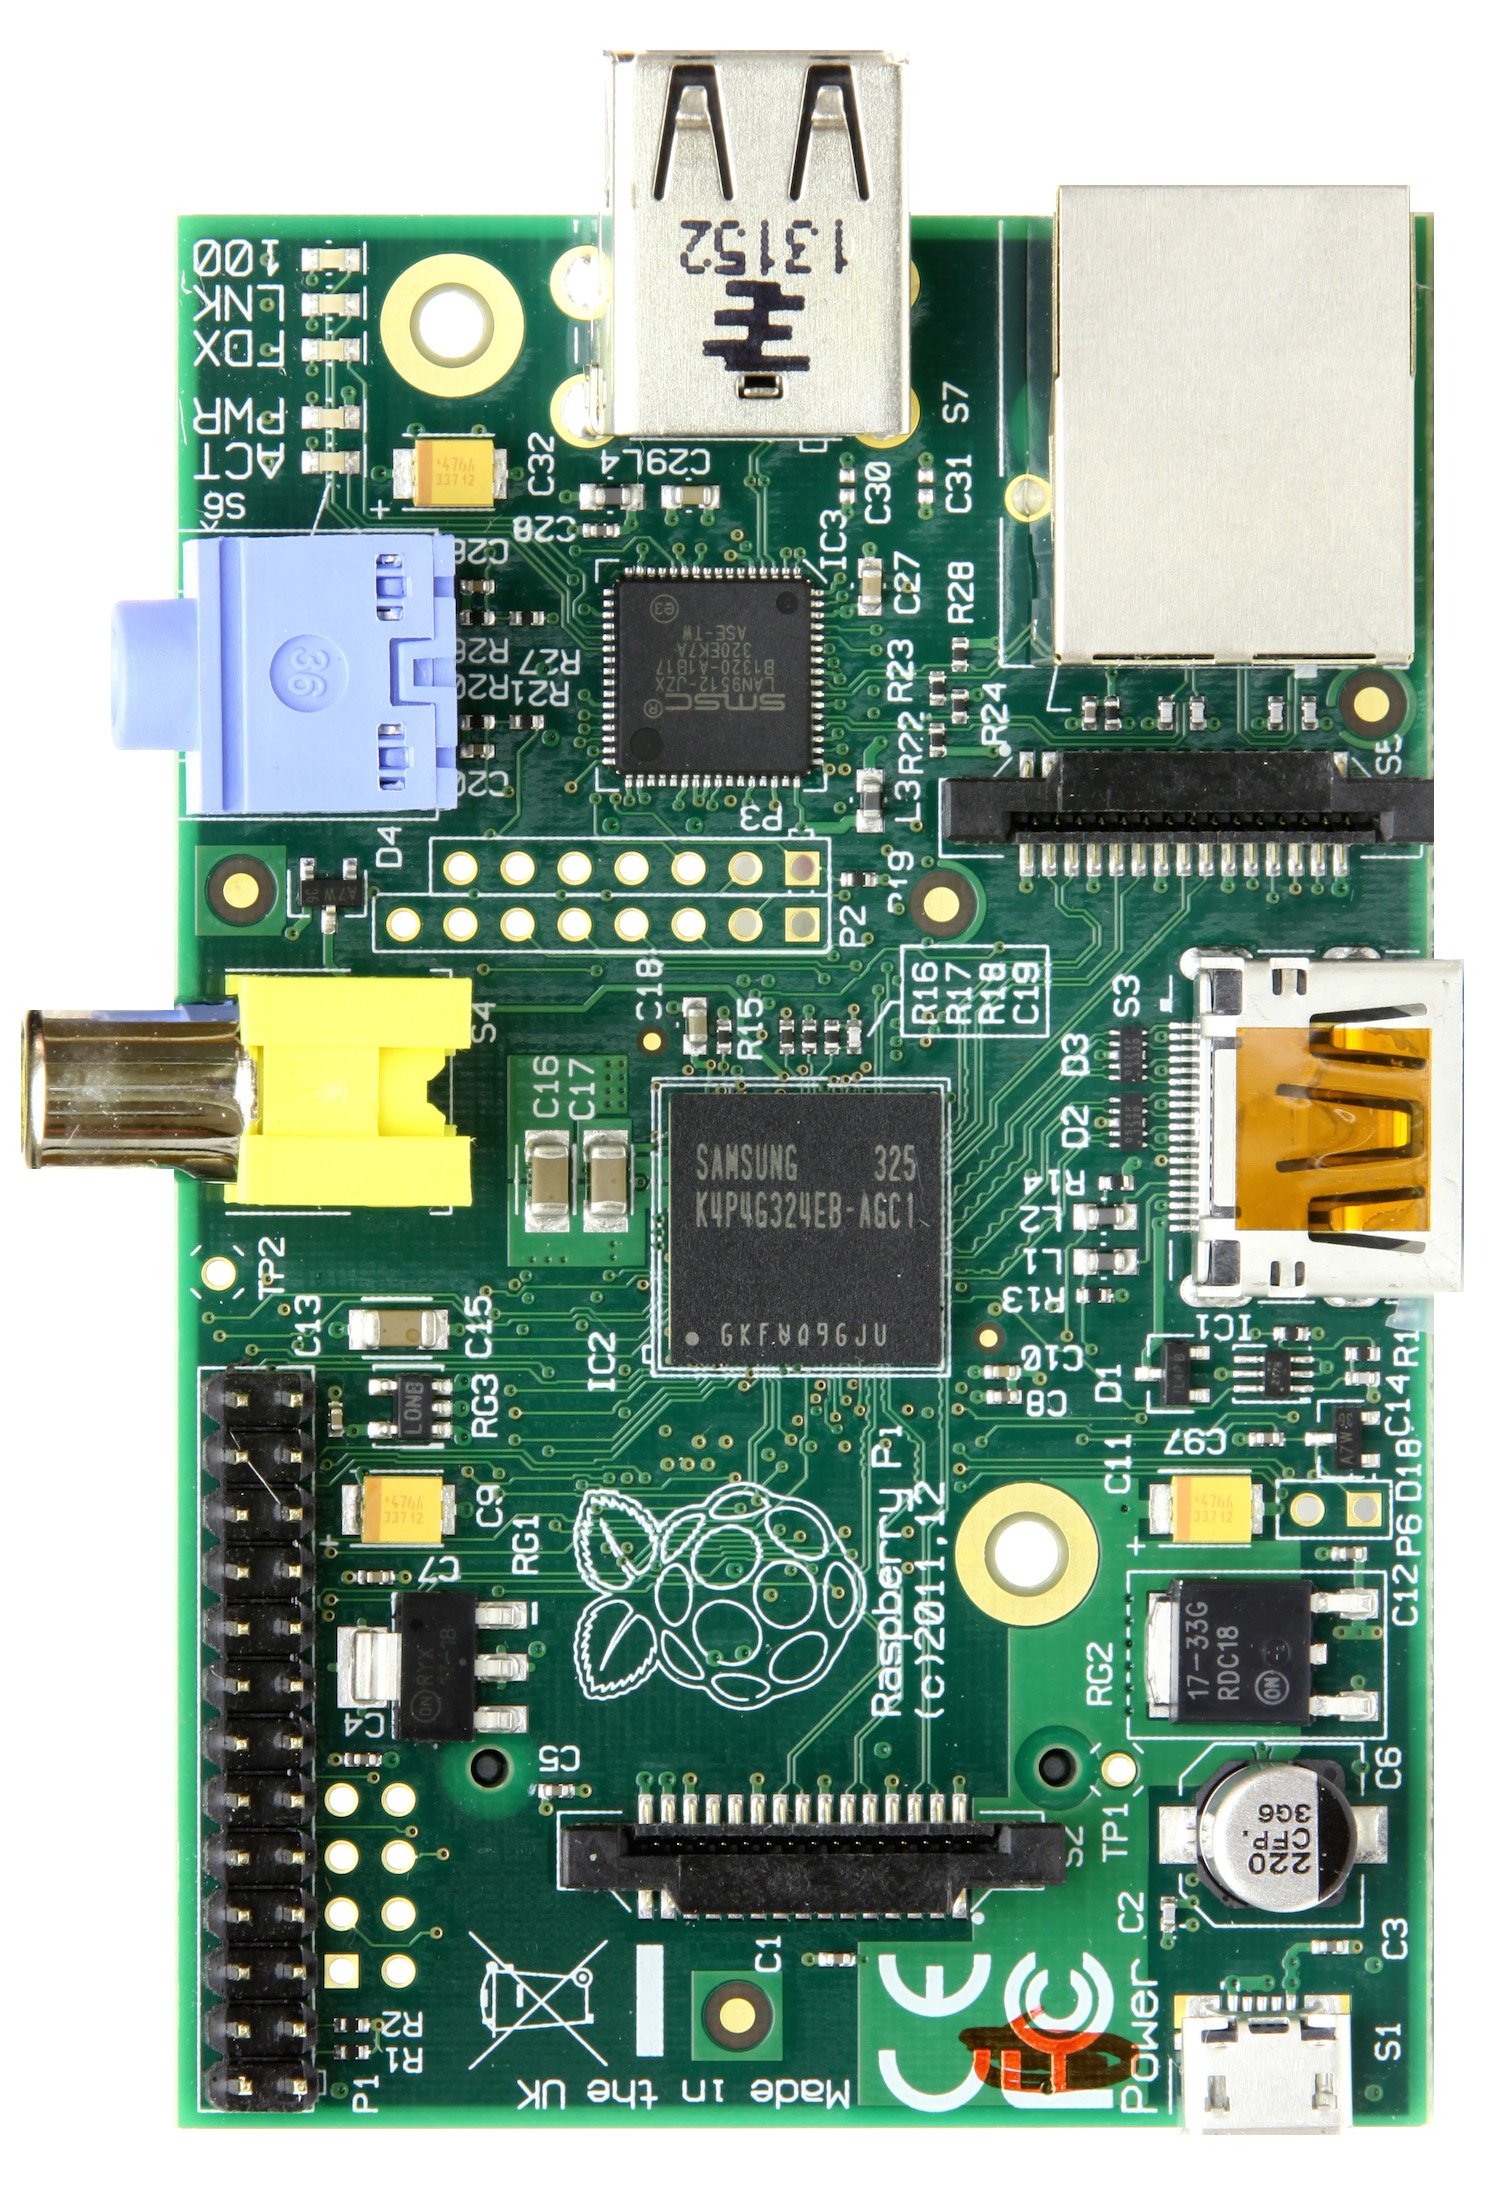
\includegraphics[width=3cm]{img/raspi.jpg}};
      \path[snake=expanding waves,segment length=2mm,segment angle=30,draw,thick,color=blue] (-1.3,0.85) -- +(-2,0);
      \draw[ultra thick] plot [smooth,tension=1.5] coordinates{(-1,-1) (-2.2, -1.6) (-4, -1.2) (-4.5, -3)};
      \node at (-4.5, -3) {\includegraphics[width=5cm]{img/Musical_keyboard.png}};
    \end{tikzpicture}
\end{frame}

\begin{frame}
	\frametitle{GPIO Keyboard with Note Velocity}
	\centering
	\begin{tikzpicture}
		\node at (-4,2) {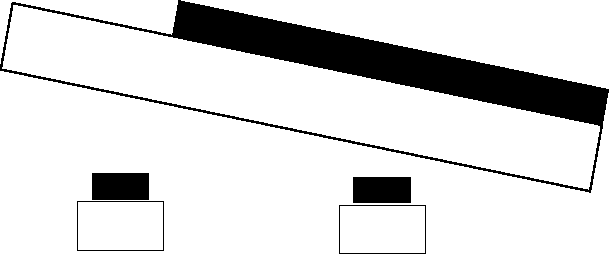
\includegraphics[width=4cm]{img/key1.pdf}};
		\node[align=left ,text width=4cm] at (1,2) { Two buttons connected \\ to GPIO ports};
		\node at (-4,0) {\includegraphics[width=4cm ]{img/key2.pdf}};
		\node[align=left ,text width=4cm] at (1,0) { Interrupt Time A};
		\node at (-4,-2) {\includegraphics[width=4cm]{img/key3.pdf}};
		\node[align=left ,text width=4cm] at (1,-2) { Interrupt Time B};
		\node[align=left ,text width=6cm] at (-1,-3.5) {  $midi\_velocity=\frac{idle\_stroke}{Time B - Time A}$};
	\end{tikzpicture}	
	
\end{frame}

\begin{frame}
  \frametitle{CMIDID Kernel Module}
  \centering
  \begin{tikzpicture}
    \node at (0, 0) {\includegraphics[width=4cm]{img/tux-on-eighth-note.jpg}};
    \node[rotate=90] at (-5, 0) {\includegraphics[width=4cm]{img/Musical_keyboard.png}};
    \node[align=center, text width=4cm] at (-3, 2.4) {GPIO Interrupts};
    \draw[ultra thick, ->] (-4, 1.5) -- (-2, 1.5);
    \draw[ultra thick, ->] (-4, .75) -- (-2, .75);
    \draw[ultra thick, ->] (-4, 0) -- (-2, 0);
    \draw[ultra thick, ->] (-4, -.75) -- (-2, -.75);
    \draw[ultra thick, ->] (-4, -1.5) -- (-2, -1.5);
    \node[align=center, text width=4cm] at (0,-2.2) {CMIDID Module};
    \draw[ultra thick, ->] (2, 0) -- (2.5, 0);
    \node[text width=2cm, draw] at (4, 0) {ALSA\\Sequencer\\Interface};
    \node[text width=4cm, align=center, rotate=270] at (2.2, -0.2) {MIDI\qquad Events};
  \end{tikzpicture}
\end{frame}
